% !TeX root = origami-activities-en.tex

\appendix

\section{Experiments with the origami axioms}\label{a.experimenting}

% Axiom 1
\begin{wrapfigure}[4]{r}{.4\textwidth}
\begin{center}
\vspace{-4ex}
\begin{tikzpicture}[scale=.9]
\coordinate (P1) at (3,6);
\coordinate (P2) at (4,3);
\fill (P1) circle (1.5pt) node[below left] {$P_1$};
\fill (P2) circle (1.5pt) node[below left] {$P_2$};
\draw[thick,dashed] ($(P1)!-.2!(P2)$) -- ($(P1)!1.5!(P2)$);
\draw[very thick,dotted,->,bend left=35] (5,5) to (2,4);
\end{tikzpicture}
\end{center}
\end{wrapfigure}
\textbf{Axiom $1$} Given two points $P_1,P_2$, there is a single fold that passes through them.

Task: Label two arbitrary points on a sheet of paper. Fold the paper so that the fold pass through the two labeled points.

\vspace{14ex}

\begin{wrapfigure}[4]{r}{.4\textwidth}
% Axiom 2
\begin{center}
\vspace{-4ex}
\begin{tikzpicture}[scale=.8]
\coordinate (P1) at (3,5);
\coordinate (P2) at (5,1);
\fill (P1) circle (1.5pt) node[above left] {$P_1$};
\fill (P2) circle (1.5pt) node[below right] {$P_2$};
\draw[thick,dashed] (2,2) -- (7,4);
\draw[very thick,dotted,->,bend left=35] (3.2,4.8) to (5,1.2);
\end{tikzpicture}
\end{center}
\end{wrapfigure}
\textbf{Axiom $2$} Given two points $P_1,P_2$, there is a single fold that places $P_1$ onto $P_2$.

Task: Label two arbitrary points on a sheet of paper. Fold the paper so that one point is placed on top of the other.

\vspace{16ex}


\begin{wrapfigure}[4]{r}{.4\textwidth}
% Axiom 3
\begin{center}
\vspace{-4ex}
\begin{tikzpicture}[scale=.8]
\draw (1,2) -- node[near start,above,xshift=-4pt] {$l_1$} (3,6);
\draw (2,1) -- node[near start,below] {$l_2$} (8,4);
\draw[thick,dashed] (1,1) -- (6,6);
\draw[very thick,dotted,->,bend left=35] (2.2,4.2) to (3.9,2.1);
\end{tikzpicture}
\end{center}
\end{wrapfigure}
\textbf{Axiom $3$} Given two lines $l_1,l_2$, there is a fold that places $l_1$ onto $l_2$.

Task: Draw two arbitrary intersecting lines on a sheet of paper. Fold the paper so that one line is placed onto the other. Is there more than one fold that can do this?

\vspace{14ex}

% Axiom 4
\begin{wrapfigure}[4]{r}{.4\textwidth}
\begin{center}
\vspace{-4ex}
\begin{tikzpicture}[scale=.9]
\coordinate (L1a) at (3,2);
\coordinate (L1b) at (5,6);
\draw[thick] (L1a) -- node[very near start,right,yshift=-4pt] {$l$} ($(L1a)!1.15!(L1b)$);
\fill (3,5.5) circle (2pt) node[above right] {$P$};
\draw[thick,dashed] (2,6) -- (8,3);
\coordinate (intersection) at (4.4,4.8);
\draw[rotate=-30] (intersection) rectangle +(8pt,8pt);
\draw[very thick,dotted,->,bend left=50] (5.4,6.3) to (3.7,3);
\end{tikzpicture}
\end{center}
\end{wrapfigure}
\textbf{Axiom $4$} Given a point $P$ and a line $l$, there is a single fold perpendicular to $l$ that passes through $P$.

Task: Draw an arbitrary line and an arbitrary point on a sheet of paper. Fold the paper so that the fold passes through the point and is perpendicular to the line.

\newpage

\begin{wrapfigure}[5]{r}{.4\textwidth}
% Axiom 5
\begin{center}
\vspace{-3ex}
\begin{tikzpicture}[scale=.6]
\coordinate (P1) at (1,4);
\coordinate (P2) at (4,3);
\fill (P1) circle (1.5pt) node[above left] {$P_1$};
\fill (P2) circle (1.5pt) node[below right] {$P_2$};
\draw[thick,dashed] (2.5,-1.5) -- (4.6,4.8); %($(3,0)!-.15!(5,6)$) -- (5,6);
\draw[thick] (1,-1) -- node[above] {$l$} ($(1,-1)!1.15!(7,2)$);
\coordinate (P3) at (7,2);
\fill (P3) circle (1.5pt) node[below right] {$P_1'$};
\draw[->,very thick,dotted,bend left=40] ($(P1)+(.2,.15)$) to ($(P3)+(-.2,.15)$);
\end{tikzpicture}
\end{center}
\end{wrapfigure}

\textbf{Axiom $5$} Given two points $P_1,P_2$ and a line $l$, there is a fold that places $P_1$ onto $l$ and passes through $P_2$.

Task: Draw two arbitrary points and an arbitrary line on a sheet of paper. Fold the paper so that the fold passes through one point and places the other point on the line.

\vspace{14ex}

\begin{wrapfigure}[8]{r}{.4\textwidth}
% Axiom 6
\begin{center}
\vspace{-6ex}
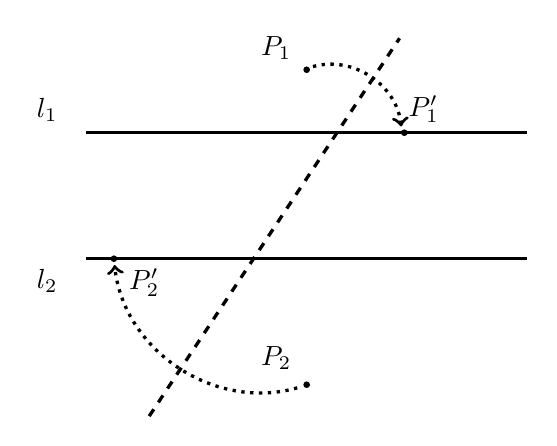
\begin{tikzpicture}[scale=.4]
\coordinate (P1) at (0,4);
\fill (P1) circle (3pt) node[above left,xshift=-2pt] {$P_1$};
\coordinate (P2) at (0,-6);
\fill (P2) circle (3pt) node[above left,xshift=-2pt,yshift=2pt] {$P_2$};
\coordinate (P1P) at (3.1,2);
\fill (P1P) circle (3pt) node[above right,xshift=-2pt] {$P_1'$};
\coordinate (P2P) at (-6.12,-2);
\fill (P2P) circle (3pt) node[below right,xshift=2pt] {$P_2'$};
\draw[very thick] (-7,2) -- node[very near start,above,xshift=-34pt] {$l_1$} (7,2);
\draw[very thick] (-7,-2) -- node[very near start,below,xshift=-34pt] {$l_2$} (7,-2);
\draw[very thick,dashed] (-5,-7) -- (2.95,5);
\draw[very thick,dotted,->,bend left=50] (.2,4.1) to (3,2.2);
\draw[very thick,dotted,->,bend left=50] (-.3,-6.1) to (-6.1,-2.2);
\end{tikzpicture}
\end{center}
\end{wrapfigure}

\textbf{Axiom $6$} Given two points $P_1,P_2$ and two lines $l_1,l_2$, there is a fold that simultaneously places $P_1$ onto $l_1$ and $P_2$ onto $l_2$.

Task: Draw two arbitrary points and two arbitrary lines on a sheet of paper. Fold the paper so that each point is one of the lines.

\vspace{16ex}

\begin{wrapfigure}{r}{.4\textwidth}
% Axiom 7
\begin{center}
\vspace{-8ex}
\begin{tikzpicture}[scale=.5]
\coordinate (P1) at (5,3);
\fill (P1) circle (2pt) node[below left] {$P$};
\coordinate (P1P) at (2.75,5.25);
\fill (P1P) circle (2pt) node[left,xshift=-4pt] {$P'$};
\draw[very thick] (1,0) -- node[very near start,right,xshift=2pt] {$l_1$} (3,6);
\draw[very thick,name path=l2] (8,3) -- node[very near start,right,xshift=-2pt,yshift=6pt] {$l_2$} (5,6);
\draw[thick] ($(1,0)!-.15!(3,6)$) -- ($(1,0)!1.34!(3,6)$);
\draw[thick] ($(8,3)!-.3!(5,6)$) -- ($(8,3)!1.65!(5,6)$);
\draw[very thick,dashed,name path=fold] (-.5,-.25) -- (7.5,7.75);
\path [name intersections = {of = fold and l2, by = {perp}}];
\draw[rotate=-45] (perp) rectangle +(8pt,8pt);
\draw[very thick,dotted,->,bend right=50] (5.1,3.2) to (3,5.2);
\end{tikzpicture}
\end{center}
\end{wrapfigure}
\textbf{Axiom $7$} Given a point $P$ and two lines $l_1,l_2$, there is a fold that places $P$ onto $l_1$ and is perpendicular to $l_2$.

Task: Draw an arbitrary point and two arbitrary lines on a sheet of paper. Fold the paper so the point is placed onto one of the lines and the fold is perpendicular to the other line.